
\begin{figure}[!htbp]
\centering
\resizebox{0.97\textwidth}{!}{%
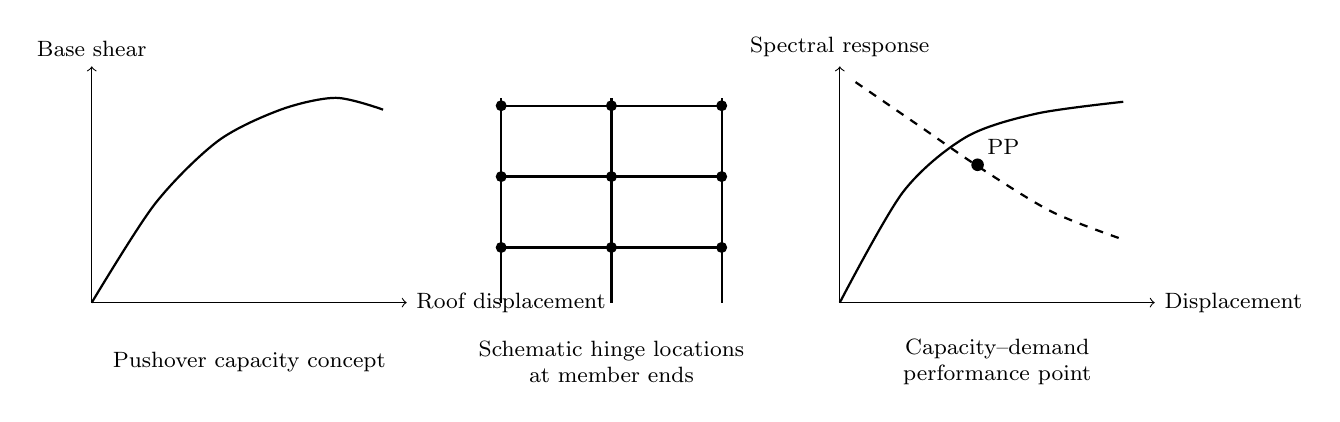
\begin{tikzpicture}[x=1cm,y=1cm,font=\footnotesize]
% panel 1 pushover
\begin{scope}[shift={(0,0)}]
\draw[->] (0,0)--(4.0,0) node[right]{Roof displacement};
\draw[->] (0,0)--(0,3.0) node[above]{Base shear};
\draw[thick] plot[smooth] coordinates {(0,0) (0.8,1.25) (1.6,2.05) (2.4,2.45) (3.1,2.60) (3.7,2.45)};
\node[align=center] at (2,-0.75) {Pushover capacity concept};
\end{scope}
% panel 2 hinges
\begin{scope}[shift={(5.2,0)}]
\foreach \x in {0,1.4,2.8}{\draw[thick] (\x,0)--(\x,2.6);}
\foreach \y in {0.7,1.6,2.5}{\draw[thick] (0,\y)--(2.8,\y);}
\foreach \x/\y in {0/0.7,1.4/0.7,2.8/0.7,0/1.6,1.4/1.6,2.8/1.6,0/2.5,1.4/2.5,2.8/2.5}{\fill (\x,\y) circle (0.07);}
\node[align=center] at (1.4,-0.75) {Schematic hinge locations\\at member ends};
\end{scope}
% panel 3 performance point
\begin{scope}[shift={(9.5,0)}]
\draw[->] (0,0)--(4.0,0) node[right]{Displacement};
\draw[->] (0,0)--(0,3.0) node[above]{Spectral response};
\draw[thick] plot[smooth] coordinates {(0,0) (0.8,1.4) (1.6,2.1) (2.5,2.4) (3.6,2.55)};
\draw[dashed,thick] plot[smooth] coordinates {(0.2,2.8) (1.0,2.25) (1.8,1.7) (2.7,1.15) (3.6,0.8)};
\fill (1.75,1.75) circle (0.08) node[above right]{PP};
\node[align=center] at (2,-0.75) {Capacity--demand\\performance point};
\end{scope}
\end{tikzpicture}%
}
\caption{Pushover analysis concepts.}
\label{fig:pushover_hinge_pp_concepts}
\end{figure}

The conceptual comparison in Figure~\ref{fig:pushover_hinge_pp_concepts} distinguishes three related but different nonlinear-response concepts. The capacity curve describes the global force--displacement response, hinge development represents localized member nonlinearity, and the performance point represents the demand--capacity state used for comparison; these quantities should therefore not be treated as interchangeable \cite{atc1996atc40,fema2005fema440,asce2017asce41}.

\FloatBarrier
